\section{Theoretische Grundlagen}

In diesem Kapitel werden die theoretischen Grundlagen erläutert, die für das Verständnis der entwickelten Middleware-Architektur erforderlich sind. Zunächst werden die verwendeten SAP-Technologien vorgestellt (Abschnitt~2.1--2.3), anschließend REST und Cloud Computing (Abschnitt~2.4--2.5), dann relevante Architekturmuster (Abschnitt~2.6) und abschließend die Microsoft Graph API für den SharePoint-Zugriff (Abschnitt~2.7).

\subsection{SAP Business Technology Platform}

Die SAP \gls{btp} ist die zentrale Entwicklungs- und Integrationsplattform von SAP für Cloud-Anwendungen \citep{sap2024btp}. Sie vereint Datenbank-, Analyse-, Integrations- und Entwicklungsfunktionen in einer einheitlichen Umgebung. Die Plattform gliedert sich in vier zentrale Bereiche:

\begin{itemize}
    \item \textbf{Database \& Data Management}: SAP HANA Cloud, Data Intelligence
    \item \textbf{Analytics}: SAP Analytics Cloud, Embedded Analytics
    \item \textbf{Application Development \& Integration}: CAP, Integration Suite, API Management
    \item \textbf{Intelligent Technologies}: AI, Machine Learning, IoT
\end{itemize}

Für die Entwicklung von Enterprise-Anwendungen stellt die BTP verschiedene Laufzeitumgebungen bereit, darunter Cloud Foundry, Kyma (Kubernetes-basiert) und ABAP Environment \citep{erl2013}.

\subsubsection{Cloud Foundry Environment}

Cloud Foundry ist eine Open-Source-Platform-as-a-Service (PaaS), die SAP als primäre Laufzeitumgebung auf der BTP anbietet \citep{cloudfoundry2024}. Sie ermöglicht das Deployment von Anwendungen in verschiedenen Programmiersprachen (Node.js, Java, Python, Go) ohne manuelle Infrastrukturverwaltung.

Die wesentlichen Konzepte von Cloud Foundry sind:

\begin{itemize}
    \item \textbf{Organizations \& Spaces}: Hierarchische Struktur zur Mandantentrennung und Umgebungsverwaltung (Dev, Test, Prod)
    \item \textbf{Buildpacks}: Automatische Erkennung und Kompilierung der Anwendung basierend auf der Programmiersprache
    \item \textbf{Services}: Verwaltete Dienste (Datenbanken, Message Queues), die an Anwendungen gebunden werden
    \item \textbf{Routes}: URL-Mappings für den externen Zugriff auf Anwendungen
\end{itemize}

Das Deployment erfolgt über das Cloud Foundry CLI mit dem Befehl \texttt{cf push}, welcher die Anwendung paketiert, einen Container erstellt und die Instanzen startet. Dieser Ansatz folgt dem \enquote{Cloud Native}-Paradigma, bei dem Anwendungen für die Cloud-Umgebung optimiert werden \citep{davis2019}.

\subsubsection{SAP Cloud ALM}

SAP \gls{calm} ist eine cloudbasierte Lösung für das Application Lifecycle Management \citep{sap2024calm}. Es unterstützt Unternehmen bei der Planung, Implementierung und dem Betrieb von SAP-Lösungen über den gesamten Lebenszyklus hinweg.

Die Kernfunktionen von SAP Cloud ALM umfassen:

\begin{itemize}
    \item \textbf{Implementation}: Projektplanung, Aufgabenverwaltung, User Stories, Anforderungsmanagement
    \item \textbf{Operations}: Monitoring, Health Management, Job Scheduling
    \item \textbf{Analytics}: Dashboards, Reports, KPIs
    \item \textbf{Process Management}: Prozessdokumentation, Fit-to-Standard-Workshops
\end{itemize}

Für diese Arbeit ist insbesondere der Implementation-Bereich relevant, da hier User Stories und deren Aufwände verwaltet werden. SAP Cloud ALM stellt diese Daten über \gls{odata}-Services bereit, was eine programmatische Integration ermöglicht. Die Verwaltung von Projektbudgets und Aufwänden entspricht dabei den etablierten Praktiken des Projektmanagements \citep{kerzner2017, pmi2021}.

\subsection{SAP Cloud Application Programming Model}

Das \gls{cap} ist ein Framework für die Entwicklung von Enterprise-Anwendungen auf der SAP \gls{btp} \citep{sap2024cap}. Es basiert auf bewährten Open-Source-Technologien und bietet eine einheitliche Programmierabstraktion für verschiedene Datenbanken und Protokolle. Das Framework folgt dem Prinzip \enquote{Convention over Configuration} und reduziert Boilerplate-Code durch deklarative Definitionen.

Die Kernprinzipien von CAP sind:

\begin{itemize}
    \item \textbf{Domain-Driven Design}: Fokus auf das Domänenmodell statt technischer Details \citep{evans2003}
    \item \textbf{Deklarative Definitionen}: Datenmodelle und Services in CDS statt imperativem Code
    \item \textbf{Best Practices}: Integrierte Unterstützung für OData, REST, Authentifizierung
    \item \textbf{Polyglotte Persistenz}: Abstraktion über verschiedene Datenbanken (SQLite, HANA, PostgreSQL)
\end{itemize}

\subsubsection{Core Data Services}

\gls{cds} ist die deklarative Modellierungssprache des \gls{cap} \citep{sap2024cds}. Mit \gls{cds} werden Datenmodelle, Services und Annotationen definiert. Die Sprache ist bewusst einfach gehalten und ähnelt SQL in ihrer Syntax.

\begin{lstlisting}[caption={Beispiel einer CDS-Service-Definition}, label={lst:cds-example}]
service BudgetService @(path: '/api/budget') {
    entity PSPElements {
        key psp      : String(50);
            name     : String(200);
            team     : String(100);
            budgetPT : Decimal(15, 2);
    }

    function getProjects() returns array of String;
    action startSession(project : String) returns { ... };
}
\end{lstlisting}

Zentrale CDS-Konzepte sind:

\begin{itemize}
    \item \textbf{Entities}: Datenstrukturen mit Schlüsselfeldern und Attributen
    \item \textbf{Services}: Gruppierung von Entities, die als API exponiert werden
    \item \textbf{Functions}: Lesende Operationen (HTTP GET)
    \item \textbf{Actions}: Schreibende Operationen (HTTP POST)
    \item \textbf{Annotations}: Metadaten für UI, Validierung, Autorisierung
\end{itemize}

Die Annotation \texttt{@cds.persistence.skip} kennzeichnet Entitäten, die nicht in einer Datenbank persistiert werden, sondern zur Laufzeit aus anderen Quellen generiert werden -- ein zentrales Konzept für die BC Middleware.

\subsubsection{Service-Implementierung in Node.js}

Die Geschäftslogik wird in JavaScript (Node.js) implementiert \citep{nodejs2024}. CAP stellt einen ereignisgesteuerten Ansatz mit Handlern für \gls{crud}-Operationen bereit. Die Ereignisse folgen einem einheitlichen Muster:

\begin{lstlisting}[caption={Event Handler in CAP}, label={lst:event-handler}]
module.exports = class BudgetService extends cds.ApplicationService {
    init() {
        // Handler fuer READ-Operation auf PSPElements
        this.on('READ', 'PSPElements', async (req) => {
            const data = await loadFromExcel();
            return data.pspElements;
        });

        // Handler fuer Custom Action
        this.on('startSession', async (req) => {
            const { project } = req.data;
            const sessionId = createSession(project);
            return { success: true, sessionId, project };
        });

        return super.init();
    }
}
\end{lstlisting}

Die verfügbaren Ereignisse sind:

\begin{itemize}
    \item \textbf{before}: Wird vor der Operation ausgeführt (Validierung, Anreicherung)
    \item \textbf{on}: Ersetzt die Standardimplementierung der Operation
    \item \textbf{after}: Wird nach der Operation ausgeführt (Transformation, Logging)
\end{itemize}

Dieses Modell ermöglicht eine saubere Trennung zwischen der deklarativen API-Definition in CDS und der imperativen Geschäftslogik in JavaScript.

\subsection{REST und RESTful APIs}

Representational State Transfer (REST) ist ein Architekturstil für verteilte Systeme, der von Roy Fielding in seiner Dissertation definiert wurde \citep{fielding2000}. REST basiert auf sechs Grundprinzipien:

\begin{enumerate}
    \item \textbf{Client-Server-Architektur}: Strikte Trennung zwischen Client (Benutzeroberfläche) und Server (Datenhaltung). Dies ermöglicht unabhängige Entwicklung und Skalierung beider Komponenten.

    \item \textbf{Zustandslosigkeit}: Jede Anfrage vom Client an den Server muss alle Informationen enthalten, die zur Verarbeitung notwendig sind. Der Server speichert keinen Client-Zustand zwischen Anfragen.

    \item \textbf{Cachebarkeit}: Antworten müssen als cachebar oder nicht-cachebar gekennzeichnet sein, um die Netzwerkeffizienz zu verbessern.

    \item \textbf{Einheitliche Schnittstelle}: Ressourcen werden über URIs identifiziert und über standardisierte HTTP-Methoden manipuliert (GET, POST, PUT, DELETE).

    \item \textbf{Schichtensystem}: Die Architektur kann aus mehreren Schichten bestehen (Load Balancer, Caches, Gateways), die für den Client transparent sind.

    \item \textbf{Code on Demand} (optional): Server können ausführbaren Code an Clients senden (z.B. JavaScript).
\end{enumerate}

Die HTTP-Methoden werden in REST wie folgt verwendet:

\begin{table}[H]
\centering
\caption{HTTP-Methoden in REST}
\label{tab:http-methods}
\begin{tabularx}{\textwidth}{llX}
\toprule
\textbf{Methode} & \textbf{CRUD} & \textbf{Beschreibung} \\
\midrule
GET & Read & Ressource abrufen (idempotent, sicher) \\
POST & Create & Neue Ressource erstellen \\
PUT & Update & Ressource vollständig ersetzen (idempotent) \\
PATCH & Update & Ressource teilweise aktualisieren \\
DELETE & Delete & Ressource löschen (idempotent) \\
\bottomrule
\end{tabularx}
\end{table}

OData baut auf diesen REST-Prinzipien auf und erweitert sie um standardisierte Query-Optionen und Metadaten \citep{oasis2020odata}. Im Vergleich zu anderen API-Stilen bietet REST eine gute Balance zwischen Einfachheit und Ausdrucksstärke, was zu seiner weiten Verbreitung im Enterprise-Umfeld beigetragen hat \citep{lauret2019}.

\subsection{Cloud Computing Grundlagen}

Cloud Computing bezeichnet die bedarfsgerechte Bereitstellung von IT-Ressourcen über das Internet \citep{erl2013}. Das National Institute of Standards and Technology (NIST) definiert in seiner weithin anerkannten Definition fünf wesentliche Charakteristiken \citep{mell2011}:

\begin{itemize}
    \item \textbf{On-Demand Self-Service}: Nutzer können Ressourcen automatisch und ohne menschliche Interaktion mit dem Anbieter bereitstellen.

    \item \textbf{Broad Network Access}: Dienste sind über Standardnetzwerke und heterogene Client-Plattformen verfügbar.

    \item \textbf{Resource Pooling}: Ressourcen des Anbieters werden gebündelt und dynamisch mehreren Nutzern zugewiesen (Multi-Tenancy).

    \item \textbf{Rapid Elasticity}: Kapazitäten können schnell und elastisch bereitgestellt werden, oft automatisch.

    \item \textbf{Measured Service}: Ressourcennutzung wird gemessen, überwacht und transparent abgerechnet.
\end{itemize}

\subsubsection{Service-Modelle}

Cloud-Dienste werden in drei Service-Modelle unterteilt:

\begin{figure}[H]
\centering
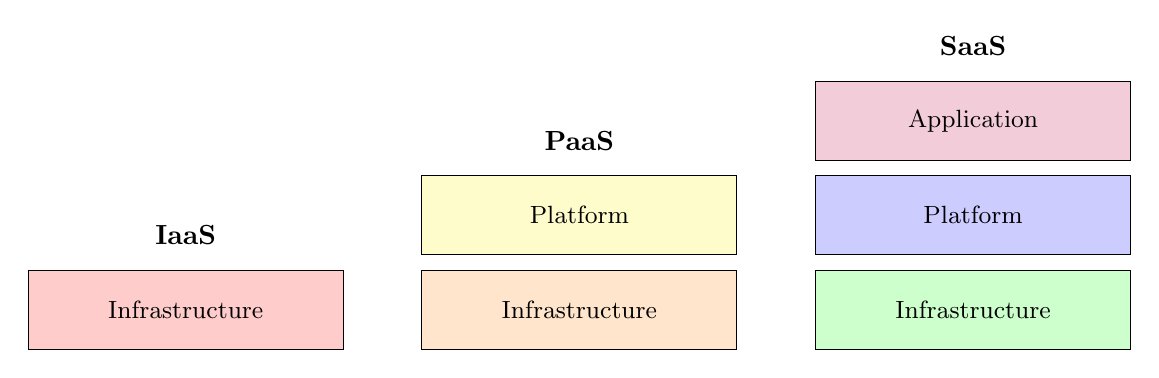
\begin{tikzpicture}[
    layer/.style={rectangle, draw, minimum width=4cm, minimum height=1cm, align=center, font=\small}
]
    % IaaS
    \node[layer, fill=red!20] (iaas-infra) at (0,0) {Infrastructure};
    \node[above] at (0,0.7) {\textbf{IaaS}};

    % PaaS
    \node[layer, fill=orange!20] (paas-infra) at (5,0) {Infrastructure};
    \node[layer, fill=yellow!20] (paas-plat) at (5,1.2) {Platform};
    \node[above] at (5,1.9) {\textbf{PaaS}};

    % SaaS
    \node[layer, fill=green!20] (saas-infra) at (10,0) {Infrastructure};
    \node[layer, fill=blue!20] (saas-plat) at (10,1.2) {Platform};
    \node[layer, fill=purple!20] (saas-app) at (10,2.4) {Application};
    \node[above] at (10,3.1) {\textbf{SaaS}};
\end{tikzpicture}
\caption{Cloud Service-Modelle}
\label{fig:cloud-models}
\end{figure}

\begin{itemize}
    \item \textbf{Infrastructure as a Service (IaaS)}: Bereitstellung von Rechenleistung, Speicher und Netzwerk. Beispiel: Amazon EC2, Microsoft Azure VMs.

    \item \textbf{Platform as a Service (PaaS)}: Bereitstellung einer Entwicklungs- und Laufzeitumgebung. Der Nutzer verwaltet nur die Anwendung. Beispiel: SAP BTP Cloud Foundry, Heroku.

    \item \textbf{Software as a Service (SaaS)}: Bereitstellung fertiger Anwendungen. Beispiel: SAP S/4HANA Cloud, Microsoft 365.
\end{itemize}

Wie in Abbildung~\ref{fig:cloud-models} dargestellt, ist die SAP BTP primär ein PaaS-Angebot, das Entwicklern eine Plattform für die Erstellung und den Betrieb von Anwendungen bereitstellt \citep{sap2024btp}.

\subsection{OData Protocol}

Das \gls{odata} ist ein offener Standard für \gls{rest}ful \gls{api}s, der von OASIS standardisiert wurde \citep{oasis2020odata}. Es definiert bewährte Praktiken für den Aufbau und die Nutzung von Web-APIs und wird von SAP als Standard für die Kommunikation zwischen Frontend und Backend verwendet \citep{sap2024odata}.

OData baut auf den Prinzipien von REST auf \citep{fielding2000} und erweitert diese um:

\begin{itemize}
    \item Einheitliche URL-Konventionen für Ressourcenzugriff
    \item Standardisierte Query-Optionen für Filterung, Sortierung, Paginierung
    \item Metadaten-Dokumente zur Selbstbeschreibung der API
    \item Batch-Requests für mehrere Operationen in einer Anfrage
\end{itemize}

\subsubsection{OData v4}

OData Version 4.01 ist die aktuelle Version des Standards und bietet gegenüber früheren Versionen verbesserte Funktionalität \citep{oasis2020odata}. Die wichtigsten Query-Optionen sind:

\begin{table}[H]
\centering
\caption{OData v4 Query-Optionen}
\label{tab:odata-options}
\begin{tabularx}{\textwidth}{lX}
\toprule
\textbf{Option} & \textbf{Beschreibung} \\
\midrule
\texttt{\$filter} & Filtern von Ergebnissen nach Bedingungen \\
\texttt{\$select} & Auswahl bestimmter Eigenschaften (Projektion) \\
\texttt{\$orderby} & Sortierung nach einer oder mehreren Eigenschaften \\
\texttt{\$top} & Begrenzung der Ergebnismenge \\
\texttt{\$skip} & Überspringen von Ergebnissen (für Paginierung) \\
\texttt{\$expand} & Einbetten verknüpfter Entitäten \\
\texttt{\$count} & Rückgabe der Gesamtanzahl der Ergebnisse \\
\bottomrule
\end{tabularx}
\end{table}

Zusätzlich zu den Query-Optionen definiert OData v4 zwei Arten von benutzerdefinierten Operationen:

\begin{itemize}
    \item \textbf{Functions}: Lesende Operationen ohne Seiteneffekte (HTTP GET). Beispiel: \texttt{getProjects()} gibt eine Liste verfügbarer Projekte zurück.
    \item \textbf{Actions}: Schreibende Operationen mit potentiellen Seiteneffekten (HTTP POST). Beispiel: \texttt{startSession(project)} erstellt eine neue Session.
\end{itemize}

SAP CAP generiert automatisch OData v4-konforme Endpunkte aus den CDS-Service-Definitionen, was die Entwicklung erheblich beschleunigt \citep{sap2024cap}.

\subsection{Architekturmuster}

Die folgenden Architekturmuster bilden das theoretische Fundament für den Entwurf der BC Middleware. Sie ermöglichen eine flexible, wartbare und erweiterbare Architektur \citep{bass2021}.

\subsubsection{Adapter Pattern}

Das Adapter-Pattern ist ein strukturelles Entwurfsmuster, das die Zusammenarbeit von Klassen mit inkompatiblen Schnittstellen ermöglicht \citep{gamma1994}. Es fungiert als Wrapper, der eine Schnittstelle in eine andere übersetzt.

\begin{figure}[H]
\centering
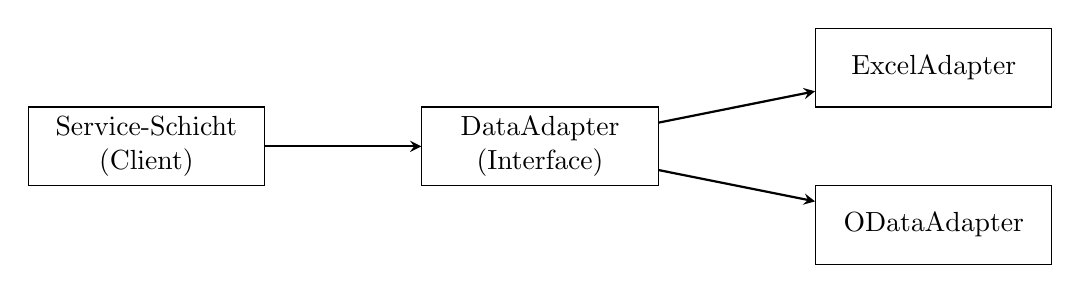
\begin{tikzpicture}[
    box/.style={rectangle, draw, minimum width=3cm, minimum height=1cm, align=center},
    arrow/.style={->, >=stealth, thick}
]
    \node[box] (client) at (0,0) {Service-Schicht\\(Client)};
    \node[box] (interface) at (5,0) {DataAdapter\\(Interface)};
    \node[box] (excel) at (10,1) {ExcelAdapter};
    \node[box] (odata) at (10,-1) {ODataAdapter};

    \draw[arrow] (client) -- (interface);
    \draw[arrow] (interface) -- (excel);
    \draw[arrow] (interface) -- (odata);
\end{tikzpicture}
\caption{Adapter-Pattern für austauschbare Datenquellen}
\label{fig:adapter-pattern}
\end{figure}

Im Kontext dieser Arbeit ermöglicht das Adapter-Pattern den Austausch der Datenquelle (Excel vs. OData-Service), ohne dass die darüberliegende Service-Schicht angepasst werden muss (siehe Abbildung~\ref{fig:adapter-pattern}). Der Adapter übersetzt die spezifische Schnittstelle der Datenquelle (Excel-Datei, REST-API) in ein einheitliches internes Datenmodell.

\subsubsection{Repository Pattern}

Das Repository-Pattern abstrahiert den Datenzugriff und stellt eine einheitliche Schnittstelle für die Geschäftslogik bereit \citep{fowler2002}. Es fungiert als Vermittler zwischen der Domänenschicht und der Datenzugriffsschicht.

Die Vorteile des Repository-Patterns sind:

\begin{itemize}
    \item \textbf{Entkopplung}: Die Geschäftslogik ist unabhängig von der konkreten Datenquelle
    \item \textbf{Testbarkeit}: Repositories können durch Mock-Objekte ersetzt werden
    \item \textbf{Zentralisierung}: Datenzugriffslogik ist an einer Stelle gebündelt
    \item \textbf{Austauschbarkeit}: Die Implementierung kann geändert werden, ohne die Geschäftslogik anzupassen
\end{itemize}

In Kombination mit dem Adapter-Pattern ergibt sich eine Architektur, bei der das Repository die Adapter-Schnittstelle nutzt und die Service-Schicht nur mit dem Repository kommuniziert.

\subsubsection{Schichtenarchitektur}

Die Schichtenarchitektur (engl. Layered Architecture) ist eines der fundamentalsten Architekturmuster in der Softwareentwicklung \citep{bass2021, starke2020}. Sie strukturiert eine Anwendung in horizontale Schichten, wobei jede Schicht eine spezifische Verantwortlichkeit hat und nur mit den direkt benachbarten Schichten kommuniziert.

\begin{figure}[H]
\centering
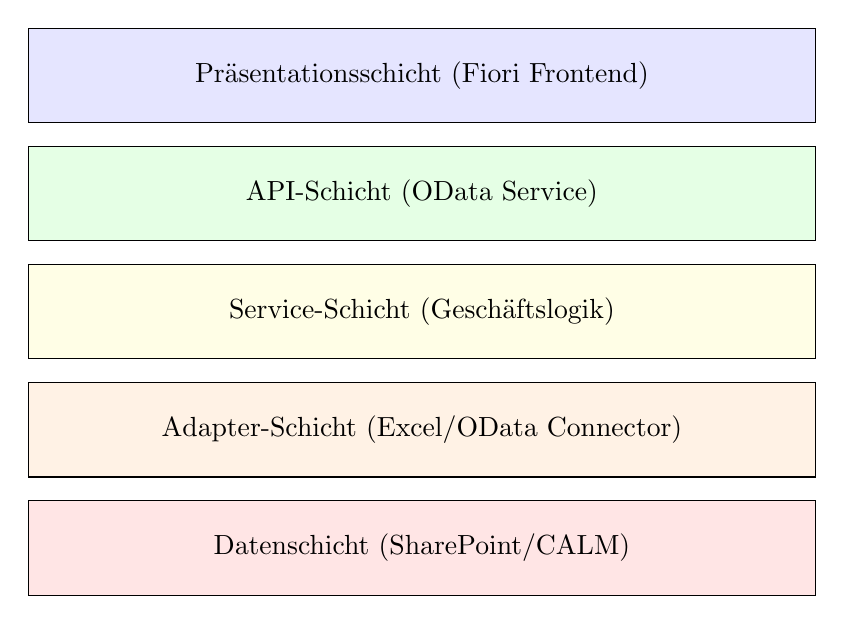
\begin{tikzpicture}[
    layer/.style={rectangle, draw, minimum width=10cm, minimum height=1.2cm, align=center}
]
    \node[layer, fill=blue!10] (pres) at (0,4) {Präsentationsschicht (Fiori Frontend)};
    \node[layer, fill=green!10] (api) at (0,2.5) {API-Schicht (OData Service)};
    \node[layer, fill=yellow!10] (service) at (0,1) {Service-Schicht (Geschäftslogik)};
    \node[layer, fill=orange!10] (adapter) at (0,-0.5) {Adapter-Schicht (Excel/OData Connector)};
    \node[layer, fill=red!10] (data) at (0,-2) {Datenschicht (SharePoint/CALM)};
\end{tikzpicture}
\caption{Schichtenarchitektur der BC Middleware}
\label{fig:layer-architecture}
\end{figure}

Die Vorteile dieser Struktur sind:

\begin{itemize}
    \item \textbf{Separation of Concerns}: Jede Schicht hat eine klar definierte Aufgabe \citep{sommerville2015}
    \item \textbf{Wartbarkeit}: Änderungen in einer Schicht haben minimale Auswirkungen auf andere Schichten
    \item \textbf{Wiederverwendbarkeit}: Schichten können in anderen Kontexten wiederverwendet werden
    \item \textbf{Testbarkeit}: Schichten können isoliert getestet werden
\end{itemize}

\subsection{Microsoft Graph API}

Die Microsoft \gls{graph} ermöglicht den programmgesteuerten Zugriff auf Microsoft 365-Dienste, einschließlich SharePoint und OneDrive \citep{microsoft2024graph}. Sie bietet einen einheitlichen Endpunkt (\texttt{https://graph.microsoft.com}) für den Zugriff auf verschiedene Microsoft-Dienste.

Für die BC Middleware sind insbesondere die SharePoint-Funktionen relevant \citep{microsoft2024sharepoint}:

\begin{itemize}
    \item Lesen von Dateien aus SharePoint-Dokumentbibliotheken
    \item Schreiben und Aktualisieren von Dateien
    \item Abrufen von Metadaten (Änderungsdatum, Autor)
\end{itemize}

\subsubsection{OAuth 2.0 Authentifizierung}

Der Zugriff auf Microsoft Graph erfordert eine Authentifizierung via OAuth 2.0 \citep{microsoft2024oauth}. Für Server-zu-Server-Kommunikation ohne Benutzerinteraktion wird der \enquote{Client Credentials Flow} verwendet:

\begin{enumerate}
    \item Die Anwendung ist in Azure Active Directory (Azure AD) registriert
    \item Die Anwendung authentifiziert sich mit Client-ID und Client-Secret
    \item Azure AD gibt ein Access Token zurück
    \item Das Token wird bei allen API-Anfragen im Authorization-Header mitgesendet
\end{enumerate}

\begin{lstlisting}[caption={Authentifizierung mit Microsoft Graph}, label={lst:ms-auth}]
const { ConfidentialClientApplication } = require('@azure/msal-node');

const msalConfig = {
    auth: {
        clientId: process.env.AZURE_CLIENT_ID,
        clientSecret: process.env.AZURE_CLIENT_SECRET,
        authority: `https://login.microsoftonline.com/${tenantId}`
    }
};

const cca = new ConfidentialClientApplication(msalConfig);
const token = await cca.acquireTokenByClientCredential({
    scopes: ['https://graph.microsoft.com/.default']
});
\end{lstlisting}

Dieser Authentifizierungsmechanismus ermöglicht es der Middleware, ohne manuelle Benutzeranmeldung auf SharePoint-Dateien zuzugreifen -- eine Voraussetzung für den automatisierten Betrieb.
